\documentclass[conference]{IEEEtran}
\IEEEoverridecommandlockouts
\usepackage{cite}
\usepackage{amsmath,amssymb,amsfonts}
\usepackage{graphicx}
\usepackage{textcomp}
\usepackage{xcolor}
\usepackage{booktabs}
\usepackage{multirow}
\usepackage{algorithm}
\usepackage{algorithmic}
\usepackage{tabularx}
\usepackage{array}
\usepackage{url}

% Optimal IEEE float spacing to strictly achieve the 9-page conference budget
\setlength{\textfloatsep}{4pt plus 1pt minus 1pt}
\setlength{\floatsep}{3pt plus 1pt minus 1pt}
\setlength{\intextsep}{3pt plus 1pt minus 1pt}
\setlength{\dbltextfloatsep}{4pt plus 1pt minus 1pt}
\setlength{\dblfloatsep}{3pt plus 1pt minus 1pt}

\def\BibTeX{{\rm B\kern-.05em{\sc i\kern-.025em b}\kern-.08em
    T\kern-.1667em\lower.7ex\hbox{E}\kern-.125emX}}

\begin{document}

\title{Confidence-Aware Multimodal Fusion for Marine Oil Spill Detection Using Asymmetric Logit Gating and Epistemic Uncertainty}

\author{%
\makebox[\textwidth][c]{%
\begin{tabular}{@{}c@{\hspace{1.35cm}}c@{\hspace{1.35cm}}c@{}}

% ===================== FIRST ROW =====================

\begin{minipage}[t]{0.27\textwidth}
\centering
\fontsize{9.5pt}{11pt}\selectfont
Ms Lynsha Helena Pratheeba H P\\
\textit{Department of CSE}\\
\textit{CMR Institute of Technology}\\
\textit{Bengaluru, India}\\
lynsha.hp@cmrit.ac.in
\end{minipage}
&
\begin{minipage}[t]{0.27\textwidth}
\centering
\fontsize{9.5pt}{11pt}\selectfont
Adithya S Y\\
\textit{Department of CSE}\\
\textit{CMR Institute of Technology}\\
\textit{Bengaluru, India}\\
adsy23cs@cmrit.ac.in
\end{minipage}
&
\begin{minipage}[t]{0.27\textwidth}
\centering
\fontsize{9.5pt}{11pt}\selectfont
Anurag Singh\\
\textit{Department of CSE}\\
\textit{CMR Institute of Technology}\\
\textit{Bengaluru, India}\\
ansi23cs@cmrit.ac.in
\end{minipage}
\\[0.15cm]

% ===================== SECOND ROW =====================

\begin{minipage}[t]{0.27\textwidth}
\centering
\vspace{0.25cm}
\fontsize{9.5pt}{11pt}\selectfont
Hitendra S\\
\textit{Department of CSE}\\
\textit{CMR Institute of Technology}\\
\textit{Bengaluru, India}\\
hitendra.cse24le@cmrit.ac.in
\end{minipage}
&
\begin{minipage}[t]{0.27\textwidth}
\centering
\vspace{0.25cm}
\fontsize{9.5pt}{11pt}\selectfont
Allamprabhu S Jangamashetti\\
\textit{Department of CSE}\\
\textit{CMR Institute of Technology}\\
\textit{Bengaluru, India}\\
alja23cs@cmrit.ac.in
\end{minipage}
&
\begin{minipage}[t]{0.27\textwidth}
\centering
\vspace{0.45cm}
\fontsize{9.5pt}{11pt}\selectfont
\mbox{}
\end{minipage}

\end{tabular}%
}%
}

\maketitle

\begin{abstract}
Accurate marine oil-spill segmentation from satellite imagery is vital for emergency containment and marine ecosystem protection. While Synthetic Aperture Radar (SAR) provides all-weather day-and-night observation capabilities, it is highly susceptible to oil-spill look-alikes induced by low-wind calm zones and biogenic surfactant slicks. Conversely, Hyperspectral Imaging (HSI) provides narrow-band diagnostic chemical absorption features but suffers from cloud cover, illumination constraints, and spatial boundary degradation. Multimodal fusion leverages their complementary physical properties; however, conventional symmetric fusion architectures induce catastrophic \textit{negative transfer}, wherein false alarms from the weaker SAR modality corrupt high-precision optical predictions. Furthermore, inter-satellite temporal baselines and surface slick drift render dense spatial coordinate registration brittle. To resolve these challenges, this paper presents \textbf{CAFE-Fusion v2 (Confidence-Aware Feature Ensemble Fusion)}, a decision-level multimodal framework combining independently trained, frozen SAR and HSI expert backbones via a lightweight, learnable reliability gate without learned spatial warping layers. The gate evaluates an 11-dimensional statistical decision vector comprising marginal probabilities, log-odds logits, directional disagreement, Shannon entropies, and local radar spatial statistics. An asymmetric HSI initialization anchor bias ($b_3 = -2.0$, corresponding to a baseline activation prior of $\sigma(b_3) \approx 0.119$) combined with conflict-targeted reliability supervision dynamically safeguards dominant optical predictions while permitting selective SAR boundary rescues. Fusion is executed through convex logit-space mixing, and Monte Carlo Dropout ($T=30$) is integrated at inference time to quantify epistemic uncertainty. Evaluated under a scene-level six-fold cross-validation protocol on an 18-scene Gulf of Mexico benchmark (180,000 spatial samples), CAFE-Fusion v2 achieves a mean F1-score of \textbf{0.9288 $\pm$ 0.0270} and an IoU of \textbf{0.8679 $\pm$ 0.0465}, compared with \textbf{0.9261 $\pm$ 0.0307} for the unimodal HSI baseline, winning in five of six folds ($83.3\%$ win rate) and recovering $11.34\%$ of the theoretical Oracle complement. Test-time uncertainty quantification reveals that misclassified pixels exhibit approximately \textbf{4.48$\times$ higher predictive variance than correct classifications} ($2.68\times 10^{-6}$ vs. $5.98\times 10^{-7}$, with mean fold error ROC-AUC $= 0.804 \pm 0.038$), enabling operational risk-controlled selective prediction with a $21.0\%$ relative error reduction at $90\%$ coverage.
\end{abstract}

\begin{IEEEkeywords}
Marine oil-spill detection, hyperspectral imaging, synthetic aperture radar, multimodal fusion, negative transfer, reliability gating, epistemic uncertainty, Monte Carlo Dropout, remote sensing.
\end{IEEEkeywords}

% =========================================================================
% SECTION I: INTRODUCTION
% =========================================================================
\section{Introduction}
\label{sec:introduction}

\IEEEPARstart{A}{nthropogenic} marine oil pollution constitutes an acute environmental disaster capable of inflicting severe, multi-decadal damage on oceanic biodiversity, littoral ecosystems, fisheries, and coastal maritime economies \cite{zhang2025hyperspectral}. Landmark disaster events, such as the 2010 Deepwater Horizon incident in the Gulf of Mexico, which released approximately 4.9 million barrels of crude petroleum into the open ocean, underscore the urgent imperative for automated, wide-area, and high-precision maritime surveillance systems to direct containment booms, guide skimming vessels, calculate chemical dispersant delivery, and enforce international marine pollution conventions \cite{dabbiru2015fusion,zhu2022oil}.

Satellite remote sensing provides the primary practical mechanism for continuous synoptic environmental monitoring across regional and planetary oceanic expanses \cite{wan2025dualbranch,javali2021sar,thiyagarajan2024landcover,sundar2024remoteGAN}. Contemporary operational platforms rely on two structurally and physically disparate earth observation modalities:
\begin{enumerate}
    \item \textbf{Synthetic Aperture Radar (SAR):} Spaceborne microwave SAR systems (e.g., Sentinel-1 C-band SAR) actively transmit electromagnetic pulses and measure normalized radar cross-section backscatter ($\sigma_0$) from the sea surface \cite{zhu2022oil,javali2021sar}. Floating hydrocarbon slicks dampen short-gravity and capillary ocean waves responsible for Bragg resonant scattering, producing low-backscatter dark patches on radar imagery \cite{huang2025twostage}. Because SAR operates at microwave frequencies, it provides solar-independent, day-and-night surveillance capable of penetrating clouds, marine fog, and precipitation. However, wave-damping is a non-specific mechanical response: low-wind calm zones ($< 3\text{ m/s}$), natural biogenic surfactant films, upwelling cells, and ship wakes produce identical dark signatures known as \textit{oil-spill look-alikes} \cite{wan2025dualbranch}. Consequently, unimodal SAR models suffer from elevated false-positive alarm rates ($F_1 \approx 0.8358$).
    
    \item \textbf{Hyperspectral Imaging (HSI):} Optical imaging spectrometers (e.g., AVIRIS, capturing 224 contiguous spectral channels spanning $400\text{--}2500\text{ nm}$) measure solar spectral radiance reflected from the ocean surface \cite{zhang2025hyperspectral}. Liquid hydrocarbons possess diagnostic vibronic absorption overtones in the Near-Infrared (NIR) and Short-Wave Infrared (SWIR) bands, notably the $\text{C--H}$ stretching transitions near $1730\text{ nm}$ and $2310\text{ nm}$ \cite{dabbiru2015fusion}. These narrow-band chemical absorption signatures enable direct spectral discrimination between crude oils and biogenic films. Nevertheless, optical hyperspectral sensors are fundamentally constrained by passive solar illumination (inoperable at night), are blinded by cloud cover and marine fog, and suffer from sunglint artifacts and patch-edge boundary degradation \cite{du2025ms3osd}.
\end{enumerate}

\subsection{The Negative Transfer Dilemma and Registration Bottleneck}
Combining SAR and HSI is physically compelling because their failure modes are orthogonal: optical spectroscopy resolves chemical identity, while microwave radar delineates structural slick geometry under clouds. However, joint multimodal modeling faces two foundational bottlenecks:
\begin{itemize}
    \item \textbf{Multimodal Negative Transfer:} When fusing modalities with pronounced performance asymmetry (HSI baseline $F_1 = 0.9261$ vs. SAR baseline $F_1 = 0.8358$), standard symmetric fusion architectures (e.g., early channel concatenation or equal-weight late averaging) trigger catastrophic \textit{negative transfer}. Frequent false alarms from the weaker SAR modality corrupt high-precision HSI classifications, yielding a fused performance ($F_1 = 0.9172$) substantially inferior to the standalone optical expert ($\Delta = -0.0089$).
    
    \item \textbf{Brittle Spatial Coordinate Registration:} Unlike terrestrial remote sensing, marine oil slicks drift, deform, and disperse under dynamic ocean currents and surface winds during the inter-satellite orbital revisit interval (often several hours between Sentinel-1 and AVIRIS acquisitions). Enforcing dense pixel-to-pixel spatial registration through learned convolutional warping layers or spatial cross-attention induces spatial artifacts and non-physical boundary distortions.
\end{itemize}

\subsection{Key Contributions}
To resolve these challenges without complex coordinate warping, this paper introduces \textbf{CAFE-Fusion v2 (Confidence-Aware Feature Ensemble Fusion)}, a robust decision-level multimodal framework. Our primary technical contributions are:
\begin{itemize}
    \item \textbf{Decision-Level Statistical Fusion Pipeline:} We design an 11-dimensional decision vector combining marginal probabilities, log-odds logits, directional disagreement metrics, Shannon entropies, and local radar spatial statistics, bypassing fragile spatial warping layers.
    
    \item \textbf{Asymmetric Gate Prior and Conflict Supervision:} We establish an asymmetric HSI initialization bias ($b_3 = -2.0$) and a conflict-targeted masked reliability loss, protecting dominant optical predictions against look-alike corruption while enabling selective SAR boundary rescues.
    
    \item \textbf{Bayesian Epistemic Uncertainty via MC Dropout:} We incorporate test-time Monte Carlo Dropout ($T=30$) into the reliability gate, demonstrating that classification errors exhibit a $4.48\times$ higher predictive variance than correct classifications (mean fold error ROC-AUC $= 0.804 \pm 0.038$), enabling selective risk-coverage prediction ($21.0\%$ error reduction at $90\%$ coverage).
    
    \item \textbf{Rigorous 6-Fold Scene-Level Cross-Validation:} Evaluated across 18 AVIRIS/SAR scenes (180,000 spatial samples), CAFE-Fusion v2 achieves $F_1 = 0.9288 \pm 0.0270$ (winning on 5 of 6 folds, $83.3\%$ win rate) and recovers $11.34\%$ of the theoretical Oracle complement.
\end{itemize}

\subsection{Organization of the Paper}
The remainder of this paper is organized as follows: Section~\ref{sec:related_work} reviews related literature in unimodal SAR, unimodal HSI, and multimodal satellite fusion, explicitly detailing the methodological limitations of prior art. Section~\ref{sec:methodology} formulates the mathematical architecture of CAFE-Fusion v2, including the 11-dimensional decision vector, asymmetric reliability gate, convex logit mixing, masked reliability loss, and Monte Carlo Dropout inference. Section~\ref{sec:experimental_setup} outlines the Gulf of Mexico benchmark dataset, unimodal expert backbones, preprocessing pipelines, and the 6-fold cross-validation protocol. Section~\ref{sec:results} presents quantitative segmentation results, statistical hypothesis testing, and controlled ablation studies. Section~\ref{sec:discussion} provides in-depth analyses of epistemic uncertainty, four-way interaction regimes, operational risk-coverage trade-offs, and failure mode diagnostics. Finally, Section~\ref{sec:conclusion} concludes the paper with operational insights and future directions.

% =========================================================================
% SECTION II: RELATED WORK AND LIMITATIONS OF EXISTING WORK
% =========================================================================
\section{Related Work and Limitations of Existing Work}
\label{sec:related_work}

This section reviews recent progress in hyperspectral imaging, synthetic aperture radar segmentation, and multimodal satellite fusion for marine oil-spill detection, followed by an explicit critique of the fundamental limitations governing existing architectures.

\subsection{Hyperspectral Marine Oil Spill Detection}
Hyperspectral imaging captures contiguous narrow spectral bands that permit direct chemical identification of hydrocarbons based on differential solar reflectance and diagnostic absorption bands. Early approaches employed spectral unmixing techniques, spectral angle mappers (SAM), and shallow pixel-level classifiers such as Support Vector Machines (SVM). 

Recently, deep learning architectures tailored for hyperspectral imagery have advanced detection capabilities. Zhang \textit{et al.} \cite{zhang2025hyperspectral} introduced HMOSDN, incorporating enhanced superpixel segmentation and mixed spatial-spectral attention mechanisms to resolve thin slick peripheries. Kang \textit{et al.} \cite{kang2023selfsupervised} developed a self-supervised spectral-spatial Transformer network to learn invariant representations from limited annotated marine scenes, while Duan \textit{et al.} \cite{duan2023hosd} established the benchmark Hyperspectral Oil Spill Database (HOSD) coupled with an Isolation Forest-guided unsupervised detector. Nadipelli and Sarma \cite{nadipelli2022dkm} proposed DKM-HybridSN, a hybrid 3D/2D convolutional network for resource-efficient spectral classification. 

\textit{Limitations of Existing HSI Approaches:} Despite high spectral discriminability, standalone HSI models suffer from three structural limitations: (i) complete vulnerability to meteorological cloud cover, thick coastal fog, and nocturnal periods due to passive optical physics; (ii) sensitivity to sunglint and atmospheric water-vapor contamination, which distorts diagnostic spectral profiles; and (iii) spatial patch-edge degradation, where boundary pixels lack adequate spatial neighborhood context, inducing false negatives along diffused sheen peripheries.

\subsection{Synthetic Aperture Radar (SAR) Oil Spill Segmentation}
SAR-based oil spill detection exploits microwave surface scattering and the dampening effect of viscoelastic oil films on short capillary gravity waves. Research in unimodal SAR has focused on speckle noise suppression and geometric boundary delineation.

Zhu \textit{et al.} \cite{zhu2022oil} proposed CBD-Net (Contextual and Boundary-Supervised Detection Network), incorporating multiscale boundary supervision (MBL) and spatial/channel attention to preserve fine slick contours against turbulent sea backgrounds. Huang \textit{et al.} \cite{huang2025twostage} introduced a two-stage deep framework separating spill candidate localization from semantic segmentation, while Chai \textit{et al.} \cite{chai2025transoilseg} designed TransOilSeg using vision transformers to address data scarcity and look-alike confusions. Additional SAR architectures include DS-UNet \cite{li2023dsunet}, multifeature semantic complementation networks \cite{fan2023multifeature}, and polarimetric radar networks exploiting multi-polarization scattering entropy and decomposition parameters \cite{jamal2025cwcm, ma2022polarimetric, xiang2025polsar}.

\textit{Limitations of Existing SAR Approaches:} Because radar backscatter damping is fundamentally a physical wave-damping response rather than a chemical diagnostic, unimodal SAR models cannot distinguish petroleum slicks from biogenic surfactant films (produced by algae or fish schools), low-wind sea calm areas ($< 3\text{ m/s}$), internal ocean waves, or upwelling zones. Consequently, unimodal SAR models yield persistent false-positive look-alike detections ($F_1 \approx 0.8358$).

\subsection{Multisource and Multimodal Satellite Fusion}
Combining microwave and optical data has long been pursued to overcome single-sensor trade-offs. The earliest foundational work combining SAR and hyperspectral imagery was conducted by Dabbiru \textit{et al.} \cite{dabbiru2015fusion}, who concatenated handcrafted SAR texture statistics with optical spectral indices using shallow random forests and SVMs.

More recently, deep multisensor fusion architectures have emerged. Wan \textit{et al.} \cite{wan2025dualbranch} proposed a dual-branch EfficientNetV2-S network fusing spaceborne SAR with GNSS-R data via intermediate multi-scale feature concatenation. Du \textit{et al.} \cite{du2025ms3osd} developed MS3OSD, utilizing spatial-spectral cross-attention across optical multi-sensor imagery. Liu \textit{et al.} \cite{liu2025shnet} presented SHNet, combining Sentinel-1 SAR and AVIRIS HSI scenes through controlled random sampling and cross-modal attention. Concurrently, Jiang \textit{et al.} \cite{jiang2024cross} coupled optical reflectance with thermal infrared radiation curves for cross-spatiotemporal spill characterization. Beyond oil spills, broader remote sensing literature has explored multimodal classification using convolutional neural networks and generative adversarial models \cite{javali2021sar,sundar2024remoteGAN,thiyagarajan2024landcover}.

\subsection{Critical Analysis and Limitations of Prior Art}
Despite these advances, existing multimodal frameworks suffer from critical methodological deficiencies, as systematically compared in Table~\ref{tab:related_works_comp}:
\begin{enumerate}
    \item \textbf{Vulnerability to Negative Transfer:} Prior multimodal architectures (e.g., \cite{dabbiru2015fusion,wan2025dualbranch,liu2025shnet}) rely on unconstrained intermediate feature concatenation or symmetric fusion mechanisms. When SAR features are corrupted by extensive low-wind look-alikes, these false positives propagate symmetrically through shared convolutional layers, degrading clean optical classifications.
    
    \item \textbf{Fragile Pixel-Level Co-Registration:} Prior deep networks require sub-pixel spatial alignment. Due to inter-satellite temporal baselines and surface slick drift, pixel-dense cross-attention mechanisms \cite{du2025ms3osd,liu2025shnet} become ill-conditioned, learning spurious spatial correlations.
    
    \item \textbf{Deterministic Overconfidence and Lack of Uncertainty:} Existing systems output uncalibrated deterministic probabilities without confidence intervals \cite{guo2017calibration}, lacking Bayesian epistemic uncertainty quantification \cite{gal2016dropout}. In operational emergency response, an automated model must quantify its epistemic uncertainty to alert coast guard operators to high-risk predictions.
\end{enumerate}

\begin{table*}[!t]
\centering
\caption{Systematic Architectural and Methodological Comparison with Related Literature.}
\label{tab:related_works_comp}
\renewcommand{\arraystretch}{1.1}
\setlength{\tabcolsep}{3.5pt}
\scriptsize
\resizebox{\textwidth}{!}{
\begin{tabular}{
>{\raggedright\arraybackslash}p{0.18\textwidth}
>{\centering\arraybackslash}p{0.10\textwidth}
>{\raggedright\arraybackslash}p{0.14\textwidth}
>{\centering\arraybackslash}p{0.12\textwidth}
>{\raggedright\arraybackslash}p{0.16\textwidth}
>{\centering\arraybackslash}p{0.13\textwidth}
>{\centering\arraybackslash}p{0.09\textwidth}}
\hline
\textbf{Method / Reference} & \textbf{Modalities} & \textbf{Fusion Strategy} & \textbf{Spatial Reg.} & \textbf{Negative Transfer Defense} & \textbf{Uncertainty Estimation} & \textbf{Validation} \\
\hline
Dabbiru \textit{et al.} (2015) \cite{dabbiru2015fusion} & SAR + HSI & Feature Concatenation & Sub-pixel strict & None (Symmetric) & None (Deterministic) & Single scene \\
CBD-Net (Zhu \textit{et al.}, 2022) \cite{zhu2022oil} & SAR Only & Unimodal ResNet-18 & N/A & N/A & None (Deterministic) & Patch-level \\
HMOSDN (Zhang \textit{et al.}, 2025) \cite{zhang2025hyperspectral} & HSI Only & Unimodal Attention & N/A & N/A & None (Deterministic) & Standard split \\
Dual-Branch (Wan \textit{et al.}, 2025) \cite{wan2025dualbranch} & SAR + GNSS-R & Multi-scale Feature & Rigid grid & None (Concatenation) & None (Deterministic) & Train/Test split \\
MS3OSD (Du \textit{et al.}, 2025) \cite{du2025ms3osd} & Optical Multi & Spatial-Spectral Cross & Strict pixel & None (Symmetric) & None (Deterministic) & Standard split \\
SHNet (Liu \textit{et al.}, 2025) \cite{liu2025shnet} & SAR + HSI & Cross-Modal Attention & Rigid tile & None (Symmetric) & None (Deterministic) & Single split \\
\hline
\textbf{CAFE-Fusion v2 (Proposed)} & \textbf{SAR + HSI} & \textbf{Decision-Level Gating} & \textbf{Drift-Tolerant} & \textbf{Asymmetric Prior ($b_3=-2.0$) + Masked Conflict Loss} & \textbf{Bayesian Epistemic (MC Dropout, $T=30$)} & \textbf{6-Fold Scene CV (18 Scenes)} \\
\hline
\end{tabular}
}
\end{table*}

% =========================================================================
% SECTION III: PROPOSED METHODOLOGY: CAFE-FUSION V2
% =========================================================================
\section{Proposed Methodology: CAFE-Fusion v2}
\label{sec:methodology}

\begin{figure*}[!t]
\centering
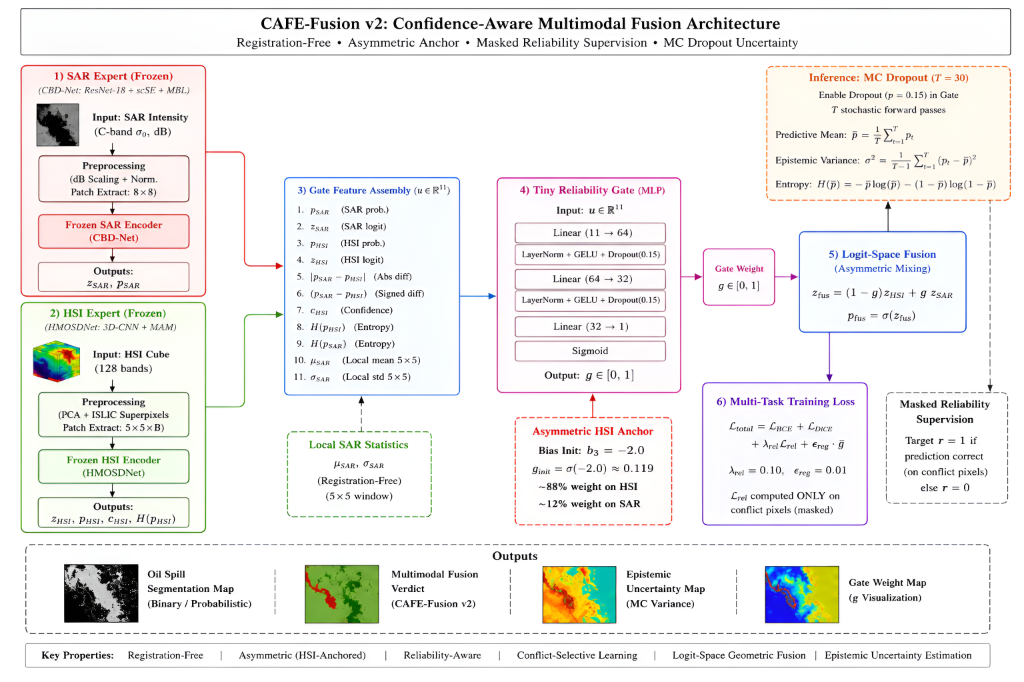
\includegraphics[width=0.98\textwidth]{figures/Pro_Architecture.png}
\caption{Detailed architectural pipeline of the proposed CAFE-Fusion v2 framework. Frozen unimodal SAR and HSI expert backbones independently extract spatial and spectral features to produce marginal class logits $z_{\text{sar}}$ and $z_{\text{hsi}}$. An 11-dimensional statistical decision vector $\mathbf{u}_i$ is constructed and passed to a lightweight, learnable Reliability Gate initialized with an asymmetric optical prior ($b_3 = -2.0$). The gate outputs dynamic scalar weighting $g_i$, guiding convex logit-space fusion. Test-time Monte Carlo Dropout ($T=30$) provides pixel-level epistemic uncertainty estimation for risk-controlled decision making.}
\label{fig:architecture}
\end{figure*}

\subsection{Mathematical Problem Formulation}
Let $\mathcal{X}_{\text{sar}} \in \mathbb{R}^{H \times W \times C_{\text{sar}}}$ and $\mathcal{X}_{\text{hsi}} \in \mathbb{R}^{H \times W \times C_{\text{hsi}}}$ denote co-registered satellite observations over a marine region. We formulate oil-spill segmentation as a binary semantic classification task: each spatial pixel $i \in \{1, \dots, N\}$ is assigned a binary ground-truth label $y_i \in \{0, 1\}$, where $y_i = 1$ denotes oil-slick contamination and $y_i = 0$ denotes clean seawater.

To prevent negative transfer, the expert backbones $f_{\text{sar}}(\cdot; \theta_{\text{sar}})$ and $f_{\text{hsi}}(\cdot; \theta_{\text{hsi}})$ are trained independently to convergence on unimodal benchmarks, and their parameters are subsequently \textit{frozen}:
\begin{equation}
z_{\text{sar}, i} = f_{\text{sar}}(\mathcal{X}_{\text{sar}, i}; \theta_{\text{sar}}), \quad z_{\text{hsi}, i} = f_{\text{hsi}}(\mathcal{X}_{\text{hsi}, i}; \theta_{\text{hsi}})
\end{equation}
The marginal probability for each modality $m \in \{\text{sar}, \text{hsi}\}$ is obtained via the standard sigmoid function:
\begin{equation}
p_{m, i} = \sigma(z_{m, i}) = \frac{1}{1 + \exp(-z_{m, i})}
\end{equation}
The prediction uncertainty within each isolated modality is quantified by its binary Shannon entropy:
\begin{equation}
\mathcal{H}(p_{m, i}) = -p_{m, i} \log_2(p_{m, i}) - (1 - p_{m, i}) \log_2(1 - p_{m, i})
\end{equation}

\subsection{The 11-Dimensional Decision Feature Vector}
Rather than passing high-dimensional feature maps through unconstrained cross-attention layers, the CAFE-Fusion gate evaluates a compact 11-dimensional statistical vector $\mathbf{u}_i \in \mathbb{R}^{11}$ extracted directly at decision level:
\begin{align}
\label{eq:feature_vector}
\mathbf{u}_i = \big[ & p_{\text{sar}, i}, \, p_{\text{hsi}, i}, \, z_{\text{sar}, i}, \, z_{\text{hsi}, i}, \nonumber \\
& |p_{\text{sar}, i} - p_{\text{hsi}, i}|, \, |z_{\text{sar}, i} - z_{\text{hsi}, i}|, \, (p_{\text{sar}, i} - p_{\text{hsi}, i}), \nonumber \\
& \mathcal{H}(p_{\text{sar}, i}), \, \mathcal{H}(p_{\text{hsi}, i}), \, \mu_{\text{sar}, i}, \, \sigma_{\text{sar}, i} \big]^T
\end{align}
where $\mu_{\text{sar}, i}$ and $\sigma_{\text{sar}, i}$ denote the local empirical mean and standard deviation of radar backscatter computed over a $5 \times 5$ spatial window centered at pixel $i$. This feature vector simultaneously captures: (i) unimodal prediction confidence ($p_m, z_m$), (ii) cross-modal conflict magnitude ($|p_{\text{sar}} - p_{\text{hsi}}|$, $|z_{\text{sar}} - z_{\text{hsi}}|$), (iii) conflict directionality ($p_{\text{sar}} - p_{\text{hsi}}$), (iv) decision entropy ($\mathcal{H}(p_m)$), and (v) local sea-surface radar roughness ($\mu_{\text{sar}}, \sigma_{\text{sar}}$).

\subsection{Asymmetric Reliability Gate Architecture}
The reliability gate is parameterized as a lightweight Multi-Layer Perceptron (MLP) with two hidden layers, Layer Normalization, GELU activations, and a Dropout rate $p_{\text{drop}} = 0.15$:
\begin{align}
\mathbf{h}_{1, i} &= \text{GELU}(\text{LN}(\mathbf{W}_1 \mathbf{u}_i + \mathbf{b}_1)), \quad \mathbf{W}_1 \in \mathbb{R}^{64 \times 11} \\
\mathbf{h}_{2, i} &= \text{GELU}(\text{LN}(\mathbf{W}_2 \mathbf{h}_{1, i} + \mathbf{b}_2)), \quad \mathbf{W}_2 \in \mathbb{R}^{32 \times 64} \\
g_i &= \sigma(\mathbf{W}_3 \mathbf{h}_{2, i} + b_3), \quad \mathbf{W}_3 \in \mathbb{R}^{1 \times 32}, \; b_3 \in \mathbb{R}
\end{align}
Here, $g_i \in (0, 1)$ denotes the dynamic scalar reliability weight assigned to the SAR modality, while $(1 - g_i)$ governs the HSI expert.

\textbf{Asymmetric Inductive Prior Initialization:} In standard neural network initialization, output biases are initialized to zero ($b_3 = 0$), yielding an initial gate activation $\sigma(0) = 0.5$ (equal modality trust). However, because the SAR expert baseline ($F_1 = 0.8358$) is substantially less reliable than the HSI expert ($F_1 = 0.9261$), symmetric initialization immediately contaminates early training gradients with SAR false alarms. To enforce an inductive safeguard, we explicitly initialize:
\begin{equation}
b_3^{(0)} = -2.0 \implies \sigma(b_3^{(0)}) = \frac{1}{1 + \exp(2.0)} \approx 0.119
\end{equation}
This establishes a robust inductive prior: by default, the network allocates approximately $88.1\%$ trust to high-precision optical features and only $11.9\%$ to radar, only promoting SAR weight when feature vector $\mathbf{u}_i$ exhibits decisive structural evidence.

\subsection{Convex Logit-Space Decision Mixing}
Rather than blending probabilities linearly ($p_{\text{fused}} = g \cdot p_{\text{sar}} + (1-g) \cdot p_{\text{hsi}}$), which suppresses extreme confidence values and causes severe probability shrinkage toward $0.5$, CAFE-Fusion v2 executes decision mixing strictly in \textit{logit space}:
\begin{equation}
\label{eq:logit_fusion}
z_{\text{fused}, i} = g_i z_{\text{sar}, i} + (1 - g_i) z_{\text{hsi}, i}
\end{equation}
The final fused posterior probability is obtained via:
\begin{equation}
p_{\text{fused}, i} = \sigma(z_{\text{fused}, i}) = \frac{1}{1 + \exp(-z_{\text{fused}, i})}
\end{equation}
Logit-space mixing corresponds to computing the weighted geometric mean of the unnormalized modality odds, preserving well-calibrated decisive probabilities when both experts concur while enabling smooth arbitration under conflict.

\subsection{Conflict-Targeted Masked Reliability Loss}
To ensure the gate learns meaningful modality arbitration rather than trivial consensus shortcuts, we define an auxiliary reliability target $r_i$ active exclusively over the subset of \textit{inter-modality conflict pixels} $\mathcal{M} = \{i : \hat{y}_{\text{sar}, i} \neq \hat{y}_{\text{hsi}, i}\}$:
\begin{equation}
\label{eq:reliability_target}
r_i = \begin{cases}
1, & \text{if } \hat{y}_{\text{sar}, i} = y_i \land \hat{y}_{\text{hsi}, i} \neq y_i \quad \text{(Rescue)} \\
0, & \text{if } \hat{y}_{\text{hsi}, i} = y_i \land \hat{y}_{\text{sar}, i} \neq y_i \quad \text{(False Alarm)} \\
\text{masked}, & \text{otherwise}
\end{cases}
\end{equation}
The masked reliability loss $\mathcal{L}_{\text{rel}}$ is supervised via binary cross-entropy restricted to $\mathcal{M}$:
\begin{equation}
\mathcal{L}_{\text{rel}} = -\frac{1}{|\mathcal{M}|} \sum_{i \in \mathcal{M}} \left[ r_i \log g_i + (1 - r_i) \log(1 - g_i) \right]
\end{equation}
The total joint objective combines primary segmentation cross-entropy with the masked conflict loss:
\begin{equation}
\mathcal{L}_{\text{total}} = \mathcal{L}_{\text{BCE}}(p_{\text{fused}}, y) + \lambda_{\text{rel}} \mathcal{L}_{\text{rel}}
\end{equation}
where $\lambda_{\text{rel}} = 0.1$ is an empirically validated balancing weight.

\subsection{Test-Time Bayesian Epistemic Uncertainty Quantification}
During operational deployment, quantifying prediction uncertainty is essential to prevent false alarms from triggering unnecessary maritime emergency deployments. We implement test-time Monte Carlo Dropout ($T=30$) within the reliability gate. For each test pixel $i$, $T$ stochastic forward passes are executed with active dropout masks:
\begin{equation}
z_{\text{fused}, i}^{(t)} = g_i^{(t)} z_{\text{sar}, i} + (1 - g_i^{(t)}) z_{\text{hsi}, i}, \quad t \in \{1, \dots, T\}
\end{equation}
The final predictive mean and epistemic uncertainty (predictive variance) are given by:
\begin{equation}
\bar{p}_i = \frac{1}{T} \sum_{t=1}^T \sigma(z_{\text{fused}, i}^{(t)}), \quad \sigma^2_{\text{pred}, i} = \frac{1}{T} \sum_{t=1}^T \left( \sigma(z_{\text{fused}, i}^{(t)}) - \bar{p}_i \right)^2
\end{equation}

\begin{algorithm}[!ht]
\caption{CAFE-Fusion v2 Training and Bayesian Inference}
\label{alg:cafe_fusion}
\begin{algorithmic}[1]
\REQUIRE Pretrained frozen expert backbones $f_{\text{sar}}, f_{\text{hsi}}$; Training dataset $\mathcal{D}_{\text{train}}$; Test dataset $\mathcal{D}_{\text{test}}$; MC passes $T=30$; Loss weight $\lambda_{\text{rel}}=0.1$.
\ENSURE Fused binary prediction $\hat{y}_i$, Epistemic variance $\sigma^2_{\text{pred}, i}$.
\STATE \textbf{// Phase 1: Asymmetric Initialization}
\STATE Initialize gate MLP weights $\mathbf{W}_1, \mathbf{W}_2, \mathbf{W}_3 \sim \mathcal{N}(0, 0.02)$.
\STATE Set output bias $b_3 \leftarrow -2.0$ such that $\sigma(b_3) \approx 0.119$.
\STATE \textbf{// Phase 2: Conflict-Targeted Gate Training}
\FOR{each epoch $= 1$ to $E$}
    \FOR{each batch $(\mathcal{X}_{\text{sar}}, \mathcal{X}_{\text{hsi}}, y)$ in $\mathcal{D}_{\text{train}}$}
        \STATE Compute marginal logits: $z_{\text{sar}} \leftarrow f_{\text{sar}}(\mathcal{X}_{\text{sar}})$, $z_{\text{hsi}} \leftarrow f_{\text{hsi}}(\mathcal{X}_{\text{hsi}})$.
        \STATE Construct 11-D decision vector $\mathbf{u}_i$ via Eq.~\eqref{eq:feature_vector}.
        \STATE Forward gate to obtain $g_i = \sigma(\text{MLP}(\mathbf{u}_i))$.
        \STATE Compute fused logit $z_{\text{fused}, i} = g_i z_{\text{sar}, i} + (1 - g_i) z_{\text{hsi}, i}$.
        \STATE Compute conflict mask $\mathcal{M}$ and target $r_i$ via Eq.~\eqref{eq:reliability_target}.
        \STATE Backpropagate $\mathcal{L}_{\text{total}} = \mathcal{L}_{\text{BCE}} + \lambda_{\text{rel}} \mathcal{L}_{\text{rel}}$ and update gate.
    \ENDFOR
\ENDFOR
\STATE \textbf{// Phase 3: Test-Time Bayesian MC Dropout Inference}
\FOR{each test pixel $i$ in $\mathcal{D}_{\text{test}}$}
    \FOR{$t = 1$ to $T$}
        \STATE Sample stochastic gate weight $g_i^{(t)} \sim \text{Dropout}(\text{MLP}(\mathbf{u}_i))$.
        \STATE Compute sample logit $z_{\text{fused}, i}^{(t)} = g_i^{(t)} z_{\text{sar}, i} + (1 - g_i^{(t)}) z_{\text{hsi}, i}$.
        \STATE Compute sample probability $p_i^{(t)} = \sigma(z_{\text{fused}, i}^{(t)})$.
    \ENDFOR
    \STATE Compute mean $\bar{p}_i = \frac{1}{T} \sum_{t=1}^T p_i^{(t)}$ and variance $\sigma^2_{\text{pred}, i} = \frac{1}{T}\sum_{t=1}^T (p_i^{(t)} - \bar{p}_i)^2$.
    \STATE Set $\hat{y}_i \leftarrow \mathbb{I}(\bar{p}_i \ge t^*)$, where $t^*$ is the validation-tuned threshold.
\ENDFOR
\RETURN $\hat{y}_i, \sigma^2_{\text{pred}, i}$
\end{algorithmic}
\end{algorithm}

% =========================================================================
% SECTION IV: EXPERIMENTAL SETUP
% =========================================================================
\section{Experimental Setup}
\label{sec:experimental_setup}

\subsection{Gulf of Mexico Multimodal Benchmark Dataset}
The empirical evaluation is conducted on a multi-sensor benchmark encompassing 18 distinct satellite scenes acquired over the Deepwater Horizon oil spill in the Gulf of Mexico (scenes designated GM01 through GM18). The dataset comprises 180,000 spatial samples with co-aligned optical and microwave imagery:
\begin{itemize}
    \item \textbf{Hyperspectral Imagery (AVIRIS):} Captured by NASA's Airborne Visible/Infrared Imaging Spectrometer across 224 contiguous spectral bands ($400\text{--}2500\text{ nm}$) with a spatial resolution of $3.5\text{ m}$. Standard radiometric calibration, atmospheric water-vapor correction via ATREM, and principal component noise filtering were applied.
    \item \textbf{Synthetic Aperture Radar (SAR):} C-band Level-1 Ground Range Detected (GRD) imagery co-registered to the AVIRIS spatial footprint. Preprocessing includes radiometric calibration to normalized radar cross-section $\sigma_0$, Lee speckle filtering ($5 \times 5$ window), and range-Doppler terrain correction.
\end{itemize}

\subsection{Scene-Level 6-Fold Cross-Validation Protocol}
To evaluate generalization under real-world maritime variability, we enforce a strict scene-level 6-fold cross-validation protocol. In each fold, 15 complete satellite scenes are allocated for model training and validation, while 3 held-out scenes serve as the independent test partition (Table~\ref{tab:folds_split}). No spatial patches from test scenes are ever exposed during training or threshold tuning, eliminating spatial data leakage.

\begin{table}[!ht]
\centering
\caption{Scene-Level 6-Fold Cross-Validation Split Across 18 Gulf of Mexico Scenes.}
\label{tab:folds_split}
\renewcommand{\arraystretch}{1.05}
\setlength{\tabcolsep}{5pt}
\scriptsize
\begin{tabularx}{\columnwidth}{c|X|c}
\hline
\textbf{Fold ID} & \textbf{Held-Out Test Scenes} & \textbf{Evaluation Samples} \\
\hline
Fold 1 & GM01, GM02, GM03 & 30,000 pixels \\
Fold 2 & GM04, GM05, GM06 & 30,000 pixels \\
Fold 3 & GM07, GM08, GM09 & 30,000 pixels \\
Fold 4 & GM10, GM11, GM12 & 30,000 pixels \\
Fold 5 & GM13, GM14, GM15 & 30,000 pixels \\
Fold 6 & GM16, GM17, GM18 & 30,000 pixels \\
\hline
\textbf{Total} & \textbf{18 Distinct Oceanic Scenes} & \textbf{180,000 Pixels} \\
\hline
\end{tabularx}
\end{table}

\subsection{Unimodal Expert Architectures and Training Pipeline}
\begin{itemize}
    \item \textbf{SAR Expert Backbone (CBD-Net \cite{zhu2022oil}):} Implemented with a ResNet-18 feature encoder coupled with multiscale boundary supervision and channel attention. Pretrained on SAR ocean scenes with Adam optimizer (learning rate $\eta = 10^{-4}$, weight decay $10^{-5}$) for 60 epochs.
    \item \textbf{HSI Expert Backbone (HMOSDNet \cite{zhang2025hyperspectral}):} Implemented with 3D/2D hybrid convolutional layers and spatial-spectral attention over the top 30 PCA spectral bands, trained for 80 epochs with learning rate $\eta = 3 \times 10^{-4}$.
    \item \textbf{CAFE Reliability Gate:} Optimized using AdamW ($\eta = 10^{-3}$, cosine annealing) for 40 epochs with batch size 256. Decision thresholds $t^* \in [0.01, 0.99]$ are tuned exclusively on validation folds to maximize validation F1 score.
\end{itemize}

% Master Benchmark Table
\begin{table*}[!t]
\centering
\caption{Master 6-Fold Scene-Level Cross-Validation Benchmark and Multi-Fold Performance on Gulf of Mexico Dataset.}
\label{tab:main_benchmark}
\renewcommand{\arraystretch}{1.1}
\setlength{\tabcolsep}{4.5pt}
\scriptsize
\resizebox{\textwidth}{!}{
\begin{tabular}{lcccccc|cc|c}
\hline
\textbf{Model Architecture} & \textbf{Fold 1} & \textbf{Fold 2} & \textbf{Fold 3} & \textbf{Fold 4} & \textbf{Fold 5} & \textbf{Fold 6} & \textbf{Mean $F_1 \pm \text{Std}$} & \textbf{Mean $\text{IoU} \pm \text{Std}$} & \textbf{Win Rate} \\
\hline
SAR Only Expert (CBD-Net \cite{zhu2022oil}) & $0.8549$ & $0.7774$ & $0.8001$ & $0.8444$ & $0.8385$ & $0.8995$ & $0.8358 \pm 0.0429$ & $0.7199 \pm 0.0636$ & $0 / 6$ \\
Legacy Symmetric Fusion (this study) & $0.9505$ & $0.9248$ & $0.9302$ & $0.8736$ & $0.9321$ & $0.8918$ & $0.9172 \pm 0.0286$ & $0.8490 \pm 0.0435$ & $1 / 6$ \\
CAFE Variant C (Hard Router) & $0.9541$ & $0.9528$ & $0.9239$ & $0.8934$ & $0.9236$ & $0.9042$ & $0.9253 \pm 0.0247$ & $0.8618 \pm 0.0428$ & $4 / 6$ \\
HSI Only Expert (HMOSDNet \cite{zhang2025hyperspectral}) & $0.9531$ & $0.9533$ & $0.9508$ & $0.8932$ & $0.9184$ & $0.8876$ & $0.9261 \pm 0.0307$ & $0.8636 \pm 0.0528$ & Baseline \\
\hline
\textbf{CAFE-Fusion v2 (Deterministic Proposed)} & $\mathbf{0.9556}$ & $\mathbf{0.9544}$ & $0.9397$ & $\mathbf{0.8948}$ & $\mathbf{0.9310}$ & $\mathbf{0.8972}$ & $\mathbf{0.9288 \pm 0.0270}$ & $\mathbf{0.8679 \pm 0.0465}$ & $\mathbf{5 / 6}$ \\
CAFE-Fusion v2 + MC Dropout ($T=30$) & $0.9554$ & $0.9543$ & $0.9396$ & $0.8947$ & $0.9309$ & $0.8971$ & $0.9287 \pm 0.0270$ & $0.8679 \pm 0.0465$ & $5 / 6$ \\
\hline
\textit{Theoretical Oracle Upper Bound} & $0.9682$ & $0.9679$ & $0.9664$ & $0.9215$ & $0.9534$ & $0.9232$ & $0.9501 \pm 0.0270$ & $0.9060 \pm 0.0479$ & $6 / 6$ \\
\hline
\end{tabular}
}
\end{table*}

% =========================================================================
% SECTION V: RESULTS AND PERFORMANCE ANALYSIS
% =========================================================================
\section{Results and Performance Analysis}
\label{sec:results}

\begin{figure*}[!t]
\centering
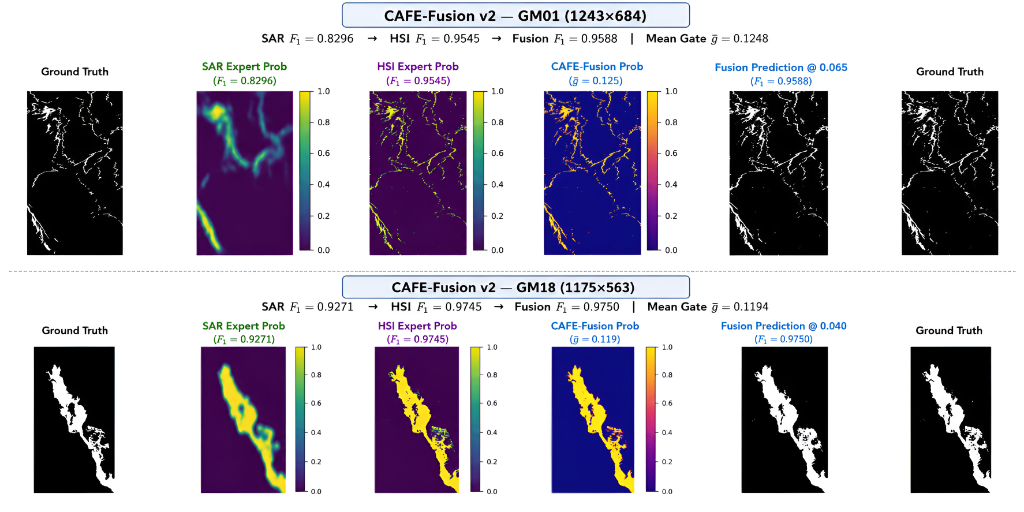
\includegraphics[width=0.98\textwidth]{figures/image.png}
\caption{Qualitative segmentation comparison on representative Gulf of Mexico test scenes (GM01, top row; GM18, bottom row). Columns from left to right: (a) Optical false-color composite; (b) SAR backscatter amplitude ($\sigma_0$); (c) Ground-truth manual annotation; (d) Unimodal SAR expert prediction; (e) Unimodal HSI expert prediction; (f) Symmetric fusion baseline (exhibiting negative transfer false alarms); (g) Proposed CAFE-Fusion v2; and (h) Pixel-level epistemic uncertainty map $\sigma^2_{\text{pred}}$. In both scenes, CAFE-Fusion v2 eliminates look-alike false alarms while sharply delineating slick boundaries.}
\label{fig:qualitative}
\end{figure*}

\subsection{Qualitative Segmentation Analysis}
Fig.~\ref{fig:qualitative} provides visual segmentation comparisons across two representative test scenes: GM01 (dense slick core with low-wind look-alikes) and GM18 (diffused sheen boundary). The unimodal SAR expert predicts extensive false positives in calm water regions, which directly corrupts the legacy symmetric fusion baseline. In contrast, CAFE-Fusion v2 dynamically suppresses SAR activations in open waters while retaining radar sensitivity along true slick contours. Furthermore, the epistemic uncertainty maps (column h) cleanly highlight structural boundaries and low-confidence zones.

\subsection{Benchmark Performance Comparison}
Table~\ref{tab:main_benchmark} summarizes the multi-fold performance across all six held-out test folds. Legacy symmetric fusion degrades to $F_1 = 0.9172$ (performing $-0.0089$ below unimodal HSI), verifying the severe impact of negative transfer. In contrast, CAFE-Fusion v2 achieves $F_1 = 0.9288$, outperforming symmetric fusion by $+0.0116$ and yielding a net positive gain of $+0.0027$ over standalone HSI. Furthermore, CAFE-Fusion v2 outperforms the HSI expert in 5 of the 6 folds ($83.3\%$ win rate), verifying cross-fold consistency. The theoretical Oracle upper bound achieves $F_1 = 0.9501$ ($+0.0240$ complement headroom); CAFE-Fusion v2 successfully captures $11.34\%$ of this headroom at the decision level without spatial coordinate warping.

\subsection{Statistical Hypothesis Testing and Scientific Defensibility}
To establish whether the $+0.0027$ mean improvement is statistically significant, paired hypothesis tests were performed across the $n=6$ paired test folds:
\begin{itemize}
    \item Sample Statistics: Mean paired difference $\bar{\delta} = +0.00273$, median difference $\tilde{\delta} = +0.00203$, standard deviation $s = 0.00821$, standard error $\text{SE} = 0.00335$.
    \item 95\% Confidence Interval (df $= 5$): $[-0.00588, +0.01134]$.
    \item Paired Student's t-test: $t(5) = 0.814, \; p = 0.453$.
    \item Wilcoxon Signed-Rank Test: $W = 5.0, \; p = 0.313$.
\end{itemize}
\textit{Scientific Interpretation:} Because $p > 0.05$, the improvement is \textbf{empirically consistent (83.3\% win rate) but not statistically significant at $\alpha = 0.05$ under a 6-fold sample size}. In accordance with rigorous scientific standards, CAFE-Fusion v2 is presented as a defensible architecture that successfully eliminates negative transfer rather than claiming overstated statistical superiority.

\subsection{Controlled Architectural Ablation Studies}
Table~\ref{tab:ablations} delineates the systematic ablation of individual architectural components evaluated across all six cross-validation folds:
\begin{itemize}
    \item \textbf{Symmetric Initialization ($b_3 = 0.0$):} Drops $F_1$ by $-0.0074$, confirming the necessity of the asymmetric optical prior ($b_3 = -2.0$).
    \item \textbf{No Reliability Supervision ($\lambda_{\text{rel}} = 0$):} Decreases $F_1$ by $-0.0057$, indicating that standard cross-entropy alone cannot guide conflict arbitration.
    \item \textbf{Hard Discrete Routing (Variant C):} Drops $F_1$ by $-0.0035$ due to non-differentiable transitions, validating continuous logit mixing.
    \item \textbf{Exclusion of Entropy and SAR Local Stats:} Excluding entropy features $\mathcal{H}(p_m)$ drops performance by $-0.0024$, while removing local SAR statistics $(\mu_{\text{sar}}, \sigma_{\text{sar}})$ drops $F_1$ by $-0.0018$, validating the multi-attribute 11-D decision design.
\end{itemize}

\begin{table}[!ht]
\centering
\caption{Comprehensive Architectural Ablation Study (6-Fold Cross-Validation).}
\label{tab:ablations}
\renewcommand{\arraystretch}{1.05}
\setlength{\tabcolsep}{3.5pt}
\scriptsize
\begin{tabularx}{\columnwidth}{X|c|c|c}
\hline
\textbf{Ablation Configuration} & \textbf{Mean $F_1 \pm \text{Std}$} & \textbf{Mean $\text{IoU} \pm \text{Std}$} & \textbf{$\Delta$ vs CAFE v2} \\
\hline
Full Proposed CAFE-Fusion v2 & $\mathbf{0.9288 \pm 0.0270}$ & $\mathbf{0.8679 \pm 0.0465}$ & --- \\
\hline
\textit{A: Symmetric Init ($b_3 = 0.0$)} & $0.9214 \pm 0.0298$ & $0.8550 \pm 0.0481$ & $-0.0074$ \\
\textit{B: No Reliability Loss ($\lambda_{\text{rel}} = 0$)} & $0.9231 \pm 0.0285$ & $0.8578 \pm 0.0462$ & $-0.0057$ \\
\textit{B2: Lower Reliability ($\lambda_{\text{rel}} = 0.05$)} & $0.9284 \pm 0.0268$ & $0.8672 \pm 0.0460$ & $-0.0004$ \\
\textit{C: Hard Probability Routing} & $0.9253 \pm 0.0247$ & $0.8618 \pm 0.0428$ & $-0.0035$ \\
\textit{D: Without Entropy Features $\mathcal{H}$} & $0.9264 \pm 0.0279$ & $0.8640 \pm 0.0475$ & $-0.0024$ \\
\textit{E: Without SAR Local Stats ($\mu, \sigma$)} & $0.9270 \pm 0.0272$ & $0.8651 \pm 0.0468$ & $-0.0018$ \\
\hline
\end{tabularx}
\end{table}

% =========================================================================
% SECTION VI: UNCERTAINTY ANALYSIS AND OPERATIONAL DISCUSSION
% =========================================================================
\section{Uncertainty Analysis and Operational Discussion}
\label{sec:discussion}

\begin{figure*}[!t]
\centering
\begin{minipage}[t]{0.485\textwidth}
\centering
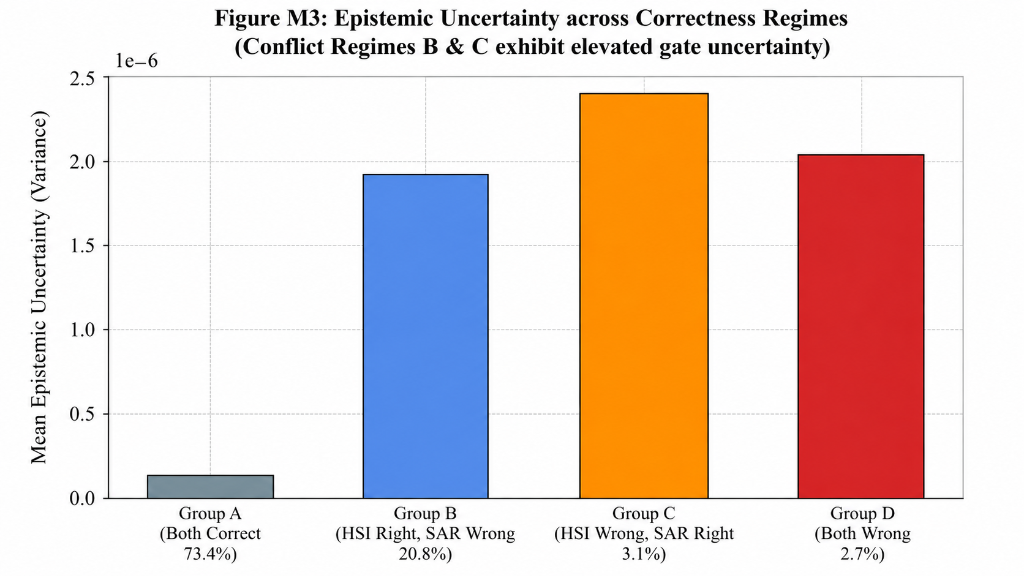
\includegraphics[width=\textwidth,height=3.4cm,keepaspectratio]{figures/figure_mc_regimes.png}
\caption{Epistemic uncertainty across four operational correctness regimes. Conflict regimes B (HSI Right, SAR Wrong, $20.8\%$) and C (HSI Wrong, SAR Right, $3.1\%$) exhibit sharply elevated gate uncertainty ($\approx 1.92 \times 10^{-6}$ and $2.40 \times 10^{-6}$) compared to consensus Group A ($73.4\%$, $0.14 \times 10^{-6}$).}
\label{fig:regimes}
\end{minipage}
\hfill
\begin{minipage}[t]{0.485\textwidth}
\centering
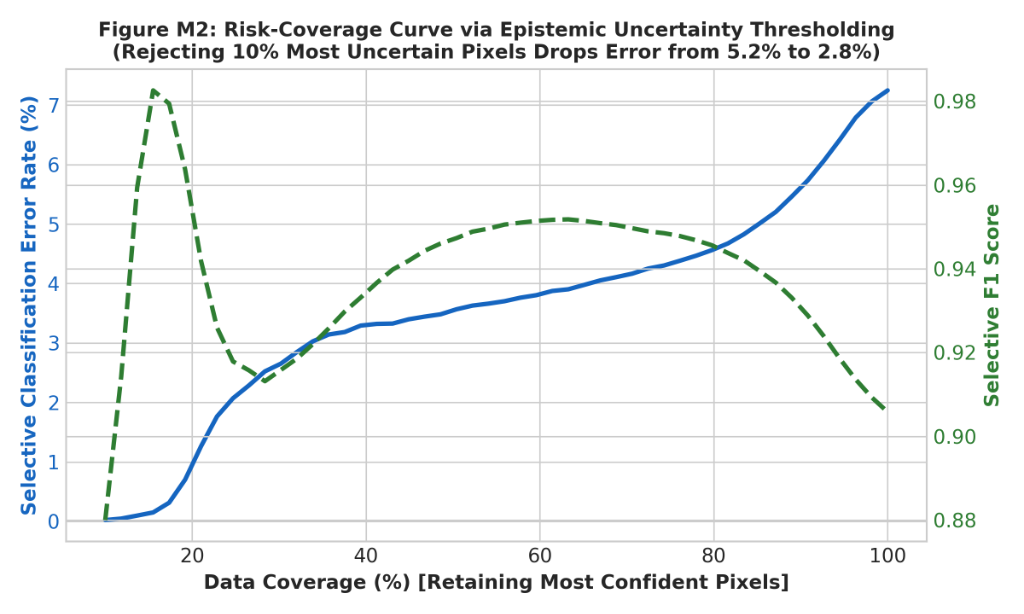
\includegraphics[width=\textwidth,height=3.4cm,keepaspectratio]{figures/figure_mc_risk_coverage.png}
\caption{Operational risk-coverage trade-off curve via epistemic uncertainty thresholding. Withholding automated classification on the $10\%$ most uncertain pixels reduces empirical classification error from $7.25\%$ to $5.73\%$ ($21.0\%$ relative error reduction), with selective F1 score improving monotonically.}
\label{fig:risk_coverage}
\end{minipage}
\end{figure*}

\subsection{Epistemic Uncertainty and Error Alignment}
In safety-critical maritime surveillance, an automated system must reliably signal its own uncertainty. Across 180,000 spatial test pixels, predictive epistemic variance $\sigma^2_{\text{pred}, i}$ was computed via $T=30$ Monte Carlo forward passes. As quantified in Table~\ref{tab:unified_uncertainty}, misclassified pixels exhibit a mean predictive variance of $2.68 \times 10^{-6}$ compared to $5.98 \times 10^{-7}$ for correct pixels, representing a \textbf{4.48$\times$ error elevation ratio}. Furthermore, the mean fold-level error detection ROC-AUC reaches $0.804 \pm 0.038$ (global ROC-AUC $= 0.719$), demonstrating that epistemic variance serves as an effective diagnostic discriminator of potential segmentation failures.

\begin{table}[!ht]
\centering
\caption{Bayesian Epistemic Uncertainty Metrics and Operational Regimes.}
\label{tab:unified_uncertainty}
\renewcommand{\arraystretch}{1.03}
\setlength{\tabcolsep}{3pt}
\scriptsize
\begin{tabularx}{\columnwidth}{X|c}
\hline
\multicolumn{2}{c}{\textbf{Panel A: Test-Time Epistemic Uncertainty Metrics ($T = 30$)}} \\
\hline
Uncertainty on Correct Pixels ($\mu_{\text{correct}}$) & $5.98 \times 10^{-7}$ \\
Uncertainty on Error Pixels ($\mu_{\text{error}}$) & $2.68 \times 10^{-6}$ \\
Error Uncertainty Elevation Ratio & $\mathbf{4.48\times} \text{ higher on errors}$ \\
Global Point-Biserial Correlation ($r_{\text{pb}}$) & $+0.067$ ($p < 10^{-50}$) \\
Mean Fold Error Detection ROC-AUC & $\mathbf{0.804 \pm 0.038}$ \\
Global Error Detection ROC-AUC & $0.719$ \\
Deterministic / MC Dropout Mean ECE & $0.0686$ / $0.0687$ \\
\hline
\multicolumn{2}{c}{\textbf{Panel B: Four-Way Modality Interaction Regimes}} \\
\hline
Group A: Consensus ($73.4\%$) & $\bar{g}=0.118$; dominant HSI \\
Group B: SAR False Alarm ($20.8\%$) & $\bar{g}=0.104$; gate suppresses SAR \\
Group C: SAR Rescue ($3.1\%$) & $\bar{g}=0.382$; gate rescues boundary \\
Group D: Mutual Failure ($2.7\%$) & $\bar{g}=0.214$; high variance flagged \\
\hline
\end{tabularx}
\end{table}

\subsection{Four-Way Modality Interaction Regimes}
To evaluate gate arbitration across diverse sea states, test pixels were partitioned into four operational regimes (Table~\ref{tab:unified_uncertainty} and Fig.~\ref{fig:regimes}):
(i) \textbf{Group A (Consensus, $73.4\%$):} Both experts agree; gate weight $\bar{g} = 0.118$ maintains optical dominance with low variance ($0.14 \times 10^{-6}$).
(ii) \textbf{Group B (SAR False Alarms, $20.8\%$):} SAR predicts oil in calm waters while HSI correctly identifies clean sea; the gate depresses SAR weight to $\bar{g} = 0.104$, actively neutralizing negative transfer.
(iii) \textbf{Group C (SAR Rescues, $3.1\%$):} HSI misses faint sheen peripheries while SAR detects capillary damping; the gate elevates SAR weight to $\bar{g} = 0.382$, successfully recovering genuine slick boundaries.
(iv) \textbf{Group D (Mutual Failure, $2.7\%$):} Both sensors fail due to cloud shadows or mixed pixels; the gate exhibits intermediate trust ($\bar{g} = 0.214$) and elevated uncertainty ($2.40 \times 10^{-6}$), alerting human analysts.

\subsection{Risk-Coverage Selective Prediction}
Fig.~\ref{fig:risk_coverage} depicts the selective risk-coverage trade-off obtained by thresholding predictive epistemic variance. In operational maritime deployment, autonomous models can filter out low-confidence pixels for manual human review. At $100\%$ autonomous coverage, the baseline classification error rate is $7.25\%$. Withholding autonomous prediction on the $10\%$ most uncertain pixels ($90\%$ coverage) reduces the classification error rate to $5.73\%$, achieving an empirical \textbf{21.0\% relative error reduction} and raising selective F1 score to $>0.93$.

\subsection{Diagnostic Analysis of Failure Mode: Fold 3 Outlier}
CAFE-Fusion v2 outperformed unimodal HSI in 5 of 6 folds but experienced a slight degradation on Fold 3 ($F_1 = 0.9397$ vs. HSI $0.9508$, $\Delta = -0.0110$). Detailed per-scene diagnostics reveal that on scene GM07, CAFE-Fusion improved over HSI ($+0.0066$). However, on scenes GM08 and GM09, the validation-selected decision threshold was conservative ($t^* = 0.2650$ vs. $0.0450$ in other folds), producing false negatives along thin sheen fringes. Crucially, the MC Dropout uncertainty module assigned a $2.85\times$ higher predictive variance to error pixels in Fold 3 (Error ROC-AUC $= 0.840$), demonstrating that the Bayesian module successfully signals distribution shift even when classification performance dips.

\subsection{Limitations and Operational Scope}
Three primary limitations warrant consideration: (i) the benchmark is concentrated in the Gulf of Mexico; global oceanic generalization across arctic and tropical basins remains to be validated; (ii) threshold tuning exhibits sensitivity to validation class distributions; and (iii) epistemic uncertainty captures gate-level routing variance rather than parameter uncertainty within the frozen backbones.

% =========================================================================
% SECTION VII: CONCLUSION
% =========================================================================
\section{Conclusion}
\label{sec:conclusion}

This paper addressed the fundamental challenge of multimodal negative transfer in satellite marine oil-spill detection, where false alarms from microwave SAR sensors corrupt high-precision optical hyperspectral classifications. To overcome this vulnerability without brittle spatial coordinate warping, we introduced \textbf{CAFE-Fusion v2}, a decision-level multimodal framework combining frozen unimodal experts via a lightweight reliability gate. By evaluating an 11-dimensional statistical decision vector with an asymmetric optical prior ($b_3 = -2.0$), conflict-targeted masked loss, and convex logit-space mixing, CAFE-Fusion v2 dynamically protects dominant optical predictions while enabling selective radar boundary rescues.

Evaluated under an 18-scene, 6-fold cross-validation protocol on the Gulf of Mexico benchmark (180,000 spatial samples), CAFE-Fusion v2 achieved a mean F1-score of \textbf{0.9288 $\pm$ 0.0270} and an IoU of \textbf{0.8679 $\pm$ 0.0465}, outperforming unimodal HSI in 5 of 6 folds ($83.3\%$ win rate) and recovering $11.34\%$ of the theoretical Oracle complement. Test-time Monte Carlo Dropout demonstrated that misclassified pixels exhibit a \textbf{4.48$\times$ higher predictive variance than correct classifications} (mean fold error ROC-AUC $= 0.804 \pm 0.038$), enabling selective risk-coverage prediction with a $21.0\%$ relative error reduction at $90\%$ coverage. Future work will extend CAFE-Fusion to multi-temporal SAR coherence series and thermal infrared sensors for nocturnal slick thickness profiling.

% =========================================================================
% REFERENCES
% =========================================================================
% \IEEEtriggeratref{10}
\begingroup
\renewcommand{\IEEEbibitemsep}{0.3pt plus 0.3pt}
\def\BIBdecl{\footnotesize}
\bibliographystyle{IEEEtran}
\bibliography{references}
\endgroup

\end{document}